\documentclass[12pt]{article}
\usepackage{graphicx}
\usepackage{geometry}
\usepackage{pdfpages}
\usepackage{titlesec}
\usepackage{centernot}
\usepackage{fancyhdr}
\usepackage{hyperref}
\usepackage{float}     % For [H] placement option in figures
% Margins
\geometry{
    a4paper,
    total={170mm,257mm},
    left=20mm,
    top=20mm,
}

\begin{document}

% Title page
\begin{titlepage}
    \centering
    \vspace*{5cm}
    
    {\Huge \textbf{MEC6602E: Transonic Aerodynamics}}\\[1.5cm]
    
    {\Large \textbf{HOMEWORK 2}}\\[2cm]
    
    {\Large Prepared by:}\\
    {\Large Kamal Jemmali 2019339}\\
    {\Large Hugo Javourez 2420717}\\[1.5cm]
    
    {\Large Submitted to :}\\
    {\Large M.Frédéric Plante. Ph.D, CPI}\\[2cm]
    
    {\Large Due date :}\\
    {\Large 28 Octobre 2024}\\
    
    \vfill
    
\includegraphics[width=0.25\textwidth]{polytechnique-signature-rgb-gauche-fr.png} % Placeholder for a logo or image (optional)
    
    \vfill
\end{titlepage}

The main goal is to simulate a shock tube, 2 nozzles case, the first one is the supersonic input and output,
and the second one is the supersonic input and subsonic output. In this report, we will show the density, rho, and mack number over x.
.Futhermore, we will show error L2 in fonction of the numbers of iterations. We will also do the simulation at differents CFL.
 

\section{Macmormack Simulations}

Before any analysis, We will show the results we got at differents parameters. 

\subsection{Shock Tube}

\subsubsection{results}

\begin{figure}[H] % Use [p] to place the figure on a separate page
    \centering
    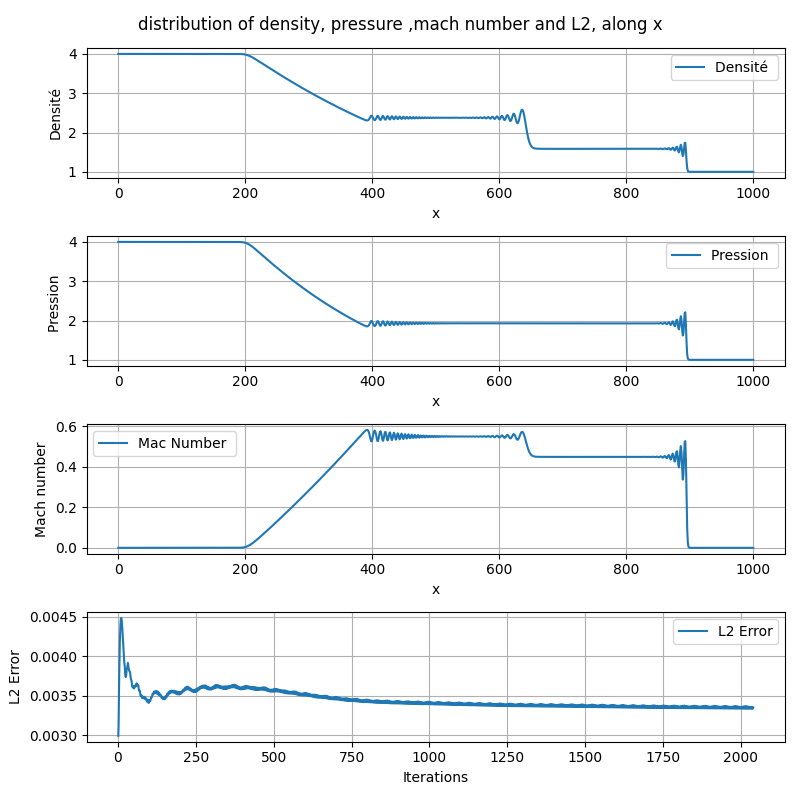
\includegraphics[width=\textwidth,height=\textheight,keepaspectratio]{PLOTS/tube_macormack_CFL25.png}
    \caption{Tube Maccormack simulation at CFL 0.25}
    \label{fig:your_label}
\end{figure}

\begin{figure}[H] % Use [p] to place the figure on a separate page
    \centering
    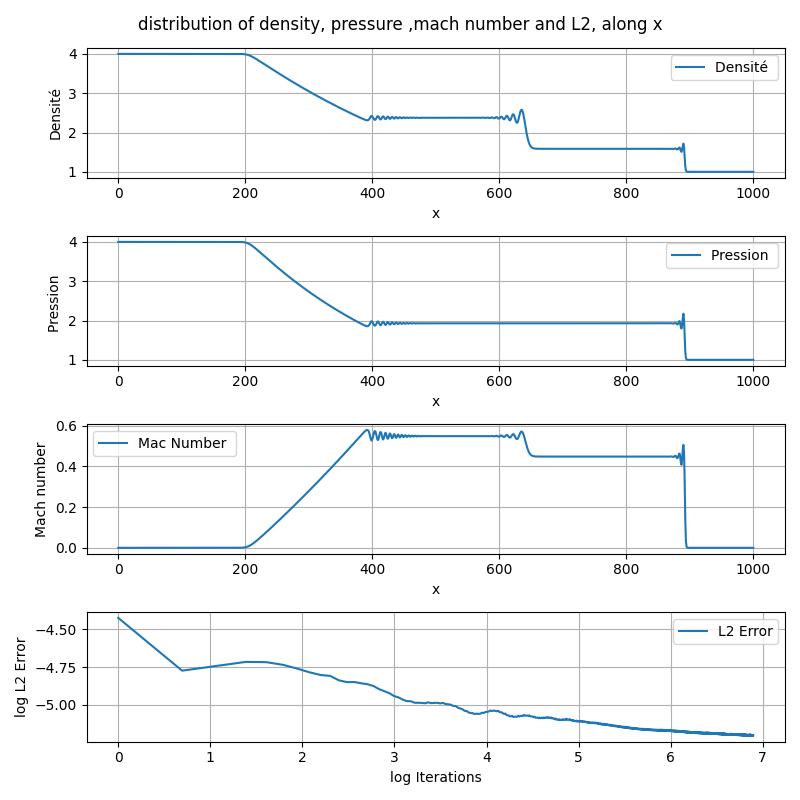
\includegraphics[width=\textwidth,height=\textheight,keepaspectratio]{PLOTS/tube_macormack_CFL05.png}
    \caption{Tube Maccormack simulation at CFL 0.50}
    \label{fig:your_label}
\end{figure}

\begin{figure}[H] % Use [p] to place the figure on a separate page
    \centering
    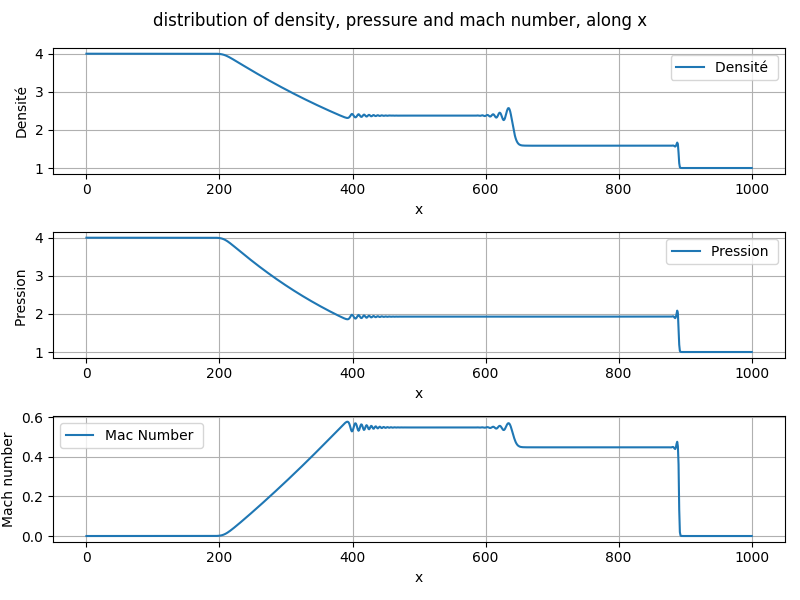
\includegraphics[width=\textwidth,height=\textheight,keepaspectratio]{PLOTS/tube_macormack_CFL75.png}
    \caption{Tube Maccormack simulation at CFL 0.75}
    \label{fig:your_label}
\end{figure}

\begin{figure}[H] % Use [p] to place the figure on a separate page
    \centering
    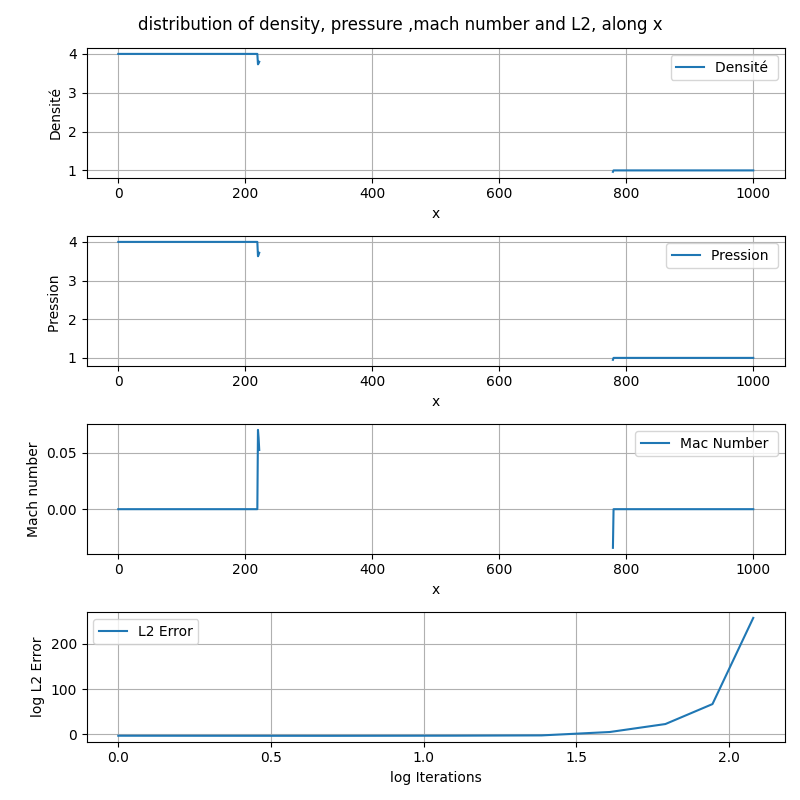
\includegraphics[width=\textwidth,height=\textheight,keepaspectratio]{PLOTS/tube_macormack_CFL110.png}
    \caption{Tube Maccormack simulation at CFL 1.1}
    \label{fig:your_label}
\end{figure}

\subsubsection{Analysis}

As we can see, for $ 0 < CFL < 1$, The scheme converge to a certain solutions that is the solution given is the .dat file
.We can also see that the scheme is stable because the L2 gets lowers when there is more iterations. As exepected, thios does 
not happen when the $CFL > 1$ Because this is an explicit scheme

\subsection{SuperSonic - Supersonic Nozzle}

\subsubsection{results}
\begin{figure}[H] % Use [p] to place the figure on a separate page
    \centering
    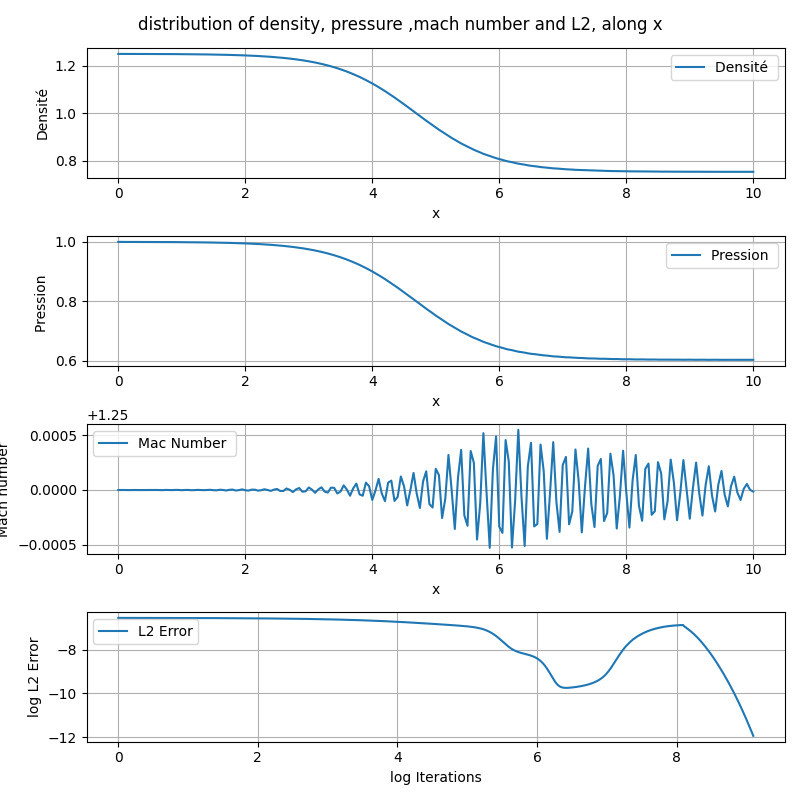
\includegraphics[width=\textwidth,height=\textheight,keepaspectratio]{PLOTS/Tuyere_super_super_Macormack_CFL050.png}
    \caption{Tuyère supersonic-supersonic at CFL = 0.5}
    \label{fig:your_label}
\end{figure}
\begin{figure}[H] % Use [p] to place the figure on a separate page
    \centering
    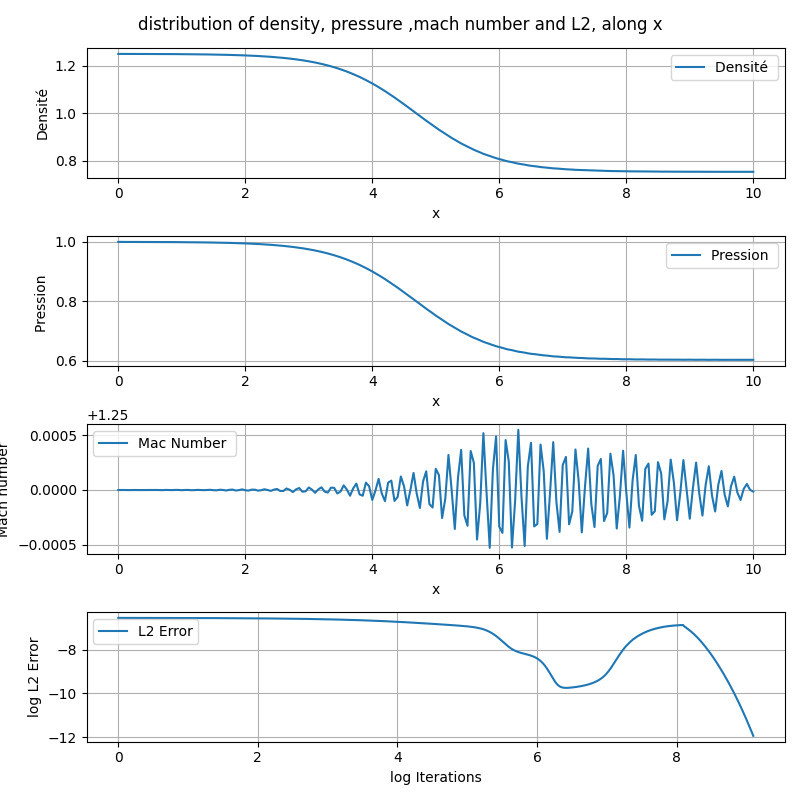
\includegraphics[width=\textwidth,height=\textheight,keepaspectratio]{PLOTS/Tuyere_super_super_Macormack_CFL050.png}
    \caption{Tuyère supersonic-supersonic at CFL = 0.5}
    \label{fig:your_label}
\end{figure}
\begin{figure}[H] % Use [p] to place the figure on a separate page
    \centering
    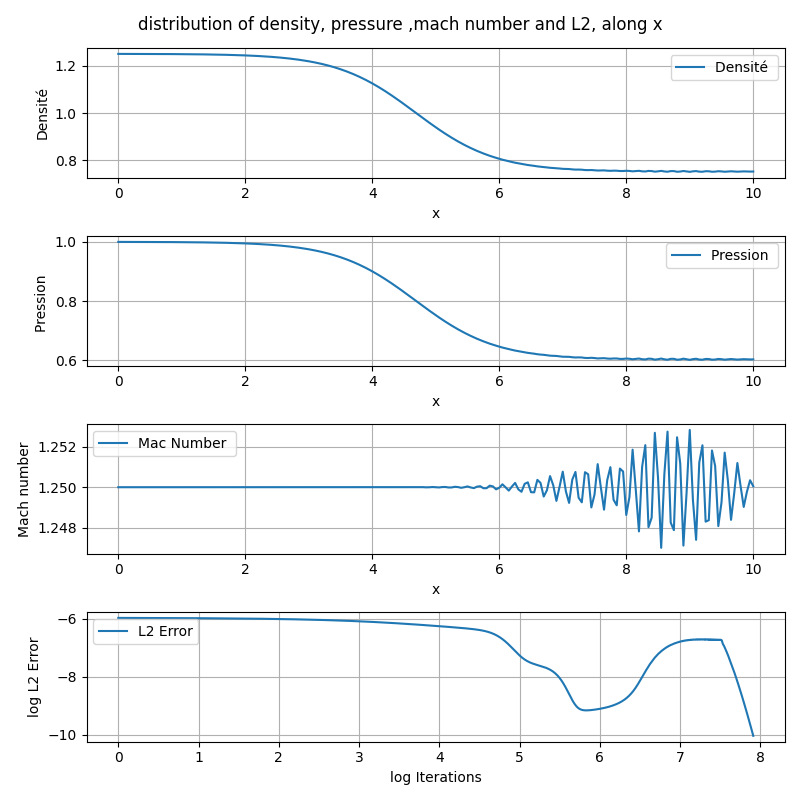
\includegraphics[width=\textwidth,height=\textheight,keepaspectratio]{PLOTS/Tuyere_super_super_Macormack_CFL090.png}
    \caption{Tuyère supersonic-supersonic at CFL = 0.90}
    \label{fig:your_label}
\end{figure}

\begin{figure}[H] % Use [p] to place the figure on a separate page
    \centering
    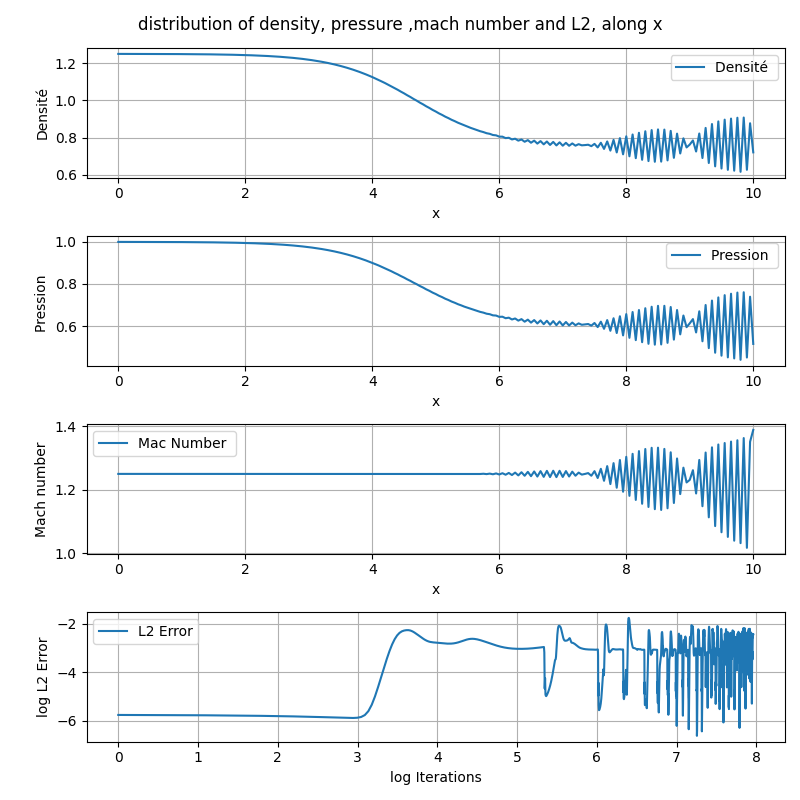
\includegraphics[width=\textwidth,height=\textheight,keepaspectratio]{PLOTS/Tuyere_super_super_Macormack_CFL110.png}
    \caption{Tuyère supersonic-supersonic at CFL = 1.10}
    \label{fig:your_label}
\end{figure}

\subsubsection{Analysis}
This is what we were expecting, a drop in density and pressure when it stabilise and the mach number becoming 1.25 everywhere. 
Careful, the mach number seems to be instable at the outlet, but please pay attention to the y-axis, you will see that its quite stable. 
As expected, the CFL number has an influence here. Its should not be higher than 1. 


\subsection{SuperSonic - Subsonic Nozzle}
\subsubsection{results}
\begin{figure}[H] % Use [p] to place the figure on a separate page
    \centering
    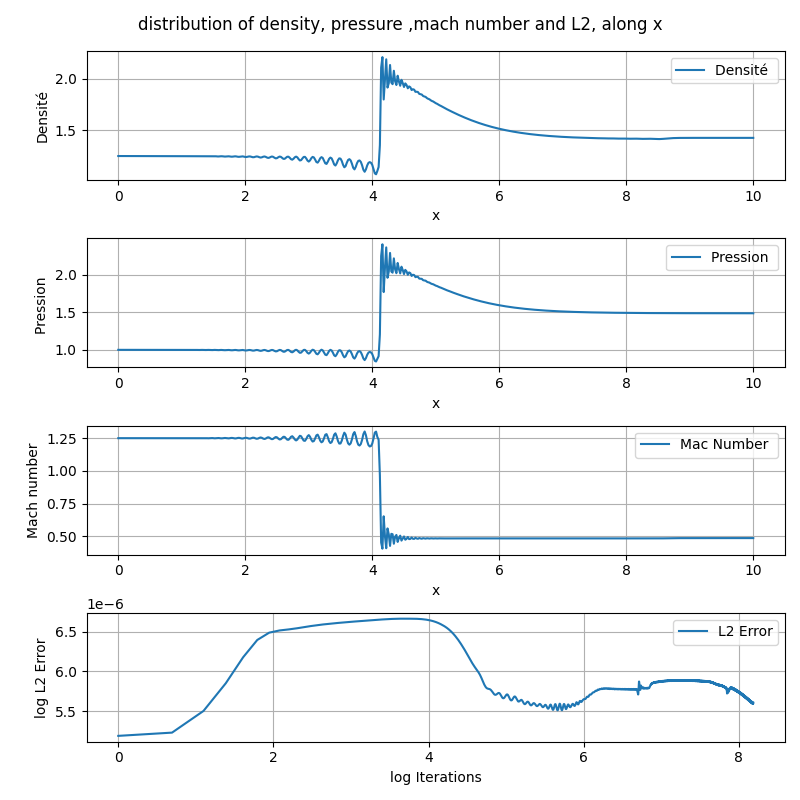
\includegraphics[width=\textwidth,height=\textheight,keepaspectratio]{PLOTS/Tuyere_super_sub_Macormack_CFL06.png}
    \caption{Tuyère supersonic-subsonic at CFL = 0.6}
    \label{fig:your_label}
\end{figure}

\begin{figure}[H] % Use [p] to place the figure on a separate page
    \centering
    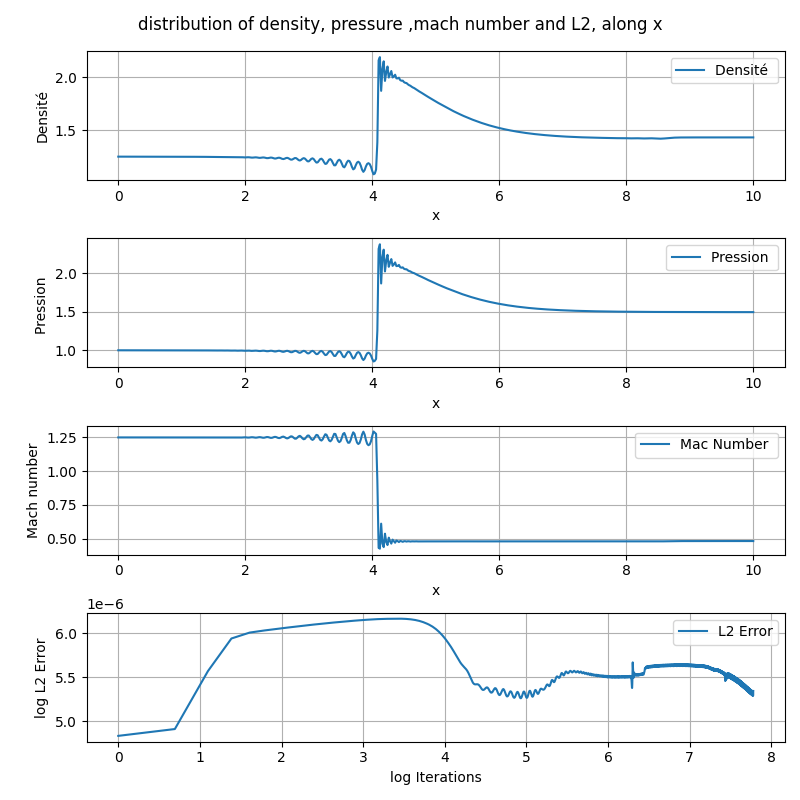
\includegraphics[width=\textwidth,height=\textheight,keepaspectratio]{PLOTS/Tuyere_super_sub_Macormack_CFL09.png}
    \caption{Tuyère supersonic-subsonic at CFL = 0.9}
    \label{fig:your_label}
\end{figure}

\begin{figure}[H] % Use [p] to place the figure on a separate page
    \centering
    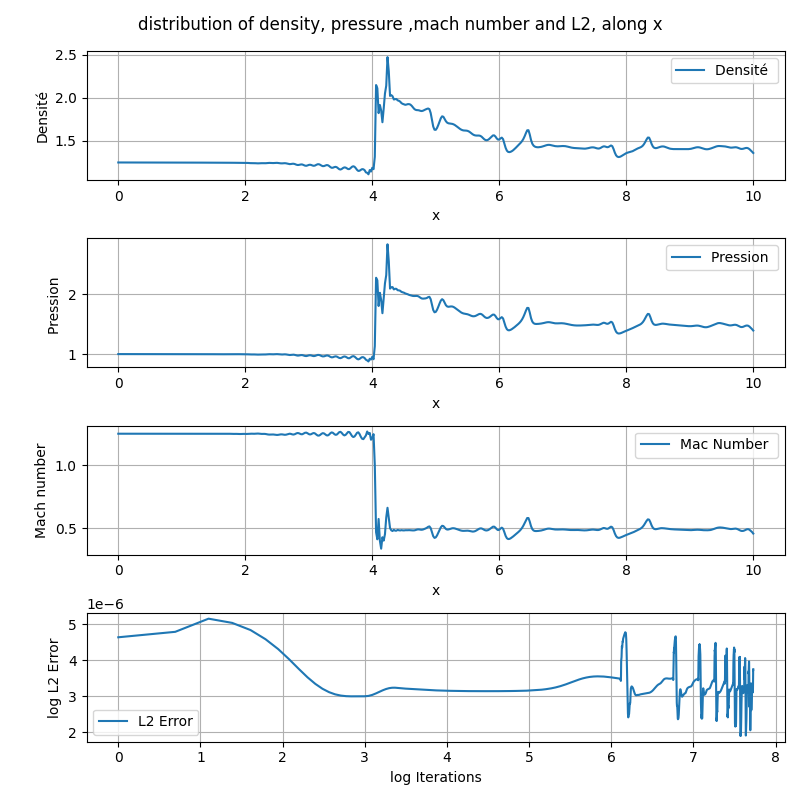
\includegraphics[width=\textwidth,height=\textheight,keepaspectratio]{PLOTS/Tuyere_super_sub_Macormack_CFL11.png}
    \caption{Tuyère supersonic-subsonic at CFL = 1.1}
    \label{fig:your_label}
\end{figure}
\subsubsection{analysis}
As we can see here, those result are the same results given at the manual, we were expecting a big drop on speed, while the pressure and density explode at the end
which is something quite logical. Here, When the $cfl>1$ we get something quite right with alot of instability, but it never diverges. 

\section{Beam Warming method}

\subsection{Tube case}

\subsubsection{results}

\begin{figure}[H] % Use [p] to place the figure on a separate page
    \centering
    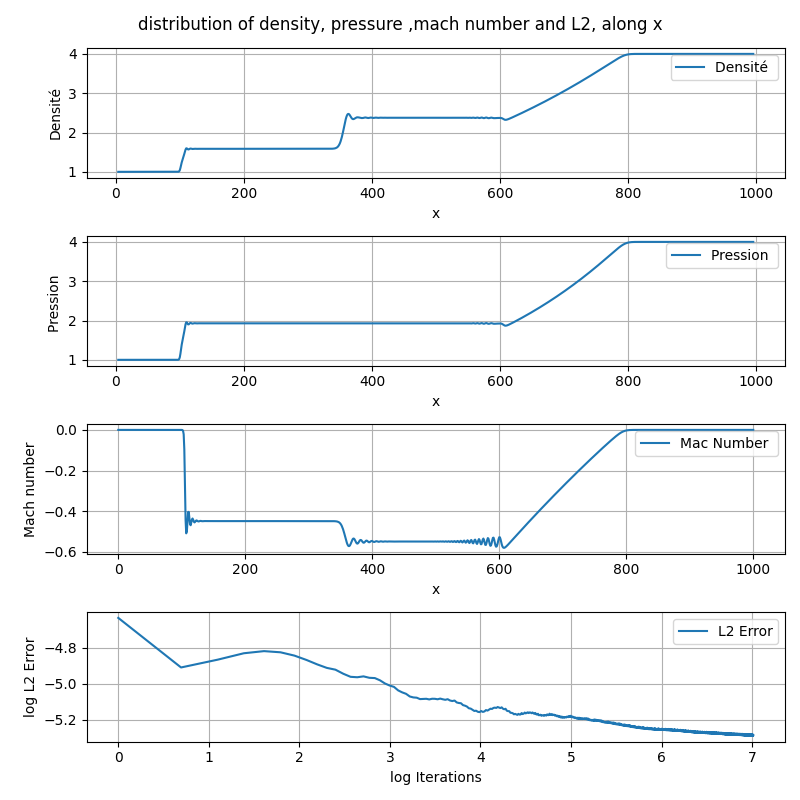
\includegraphics[width=\textwidth,height=\textheight,keepaspectratio]{PLOTS/Tube_Beam_CFL040.png}
    \caption{tube at CFL = 0.40}
    \label{fig:your_label}
\end{figure}

\begin{figure}[H] % Use [p] to place the figure on a separate page
    \centering
    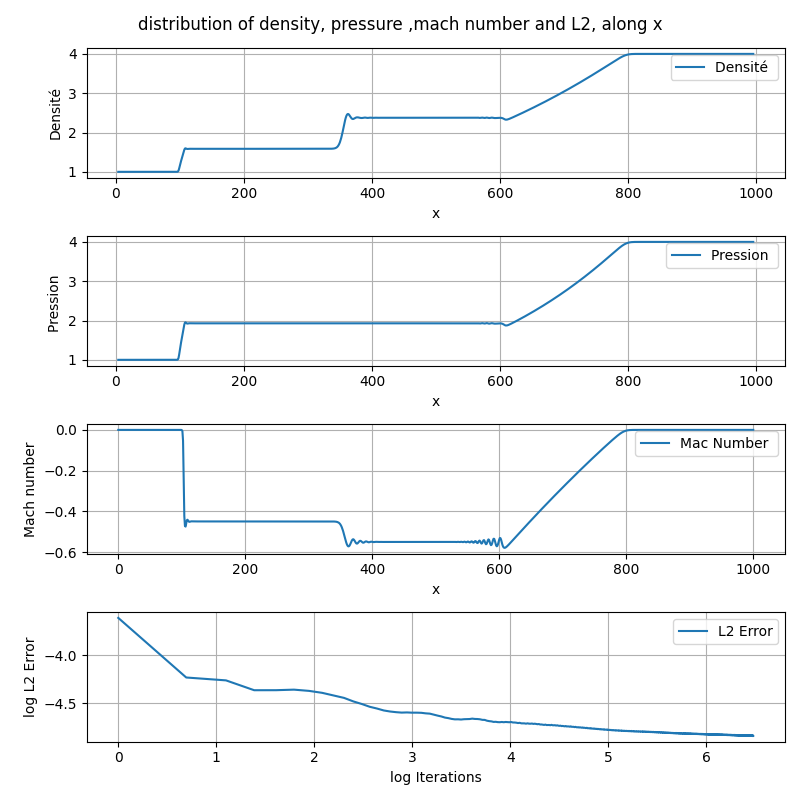
\includegraphics[width=\textwidth,height=\textheight,keepaspectratio]{PLOTS/Tube_Beam_CFL075.png}
    \caption{tube at CFL = 0.75}
    \label{fig:your_label}
\end{figure}



\begin{figure}[H] % Use [p] to place the figure on a separate page
    \centering
    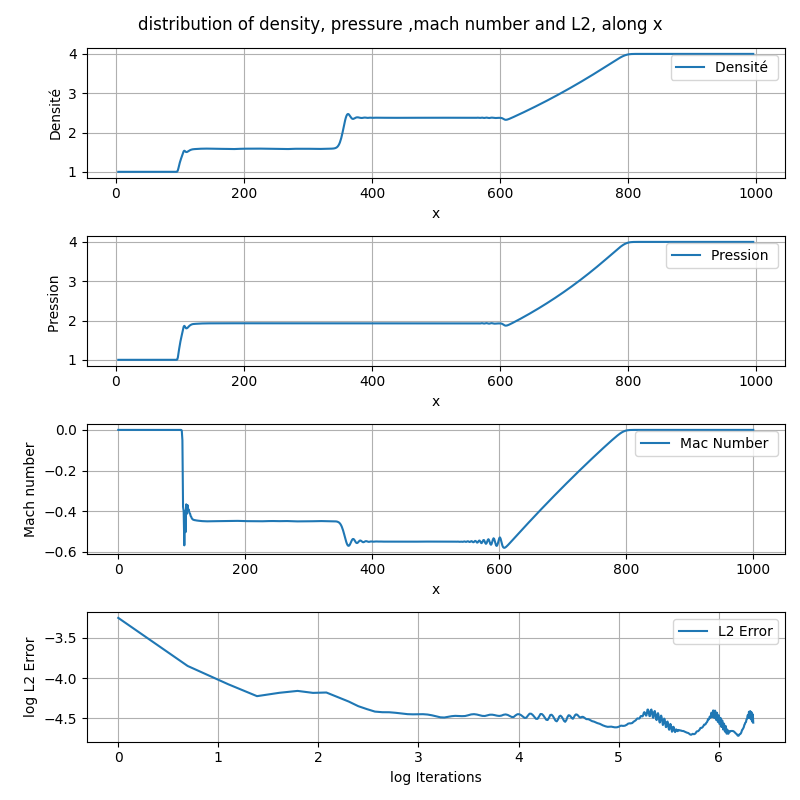
\includegraphics[width=\textwidth,height=\textheight,keepaspectratio]{PLOTS/Tube_Beam_CFL110.png}
    \caption{tube at CFL = 1.10}
    \label{fig:your_label}
\end{figure}

\subsubsection{Analysis}

There is two major element to notice with the beam-Warming method. First of all, There is much less oscillations
of the explosion point thanks to the dissipative term. Second of all, The scheme works even if the $CFL > 1.0$. Thanks to the 
the fact that the beam-warming method is an implicit scheme. We can see here that the number of oscillation gets lower when
CFL get lower too. 

\subsection{SuperSonic - Supersonic nozzles}


\subsubsection{Results}
\begin{figure}[H] % Use [p] to place the figure on a separate page
    \centering
    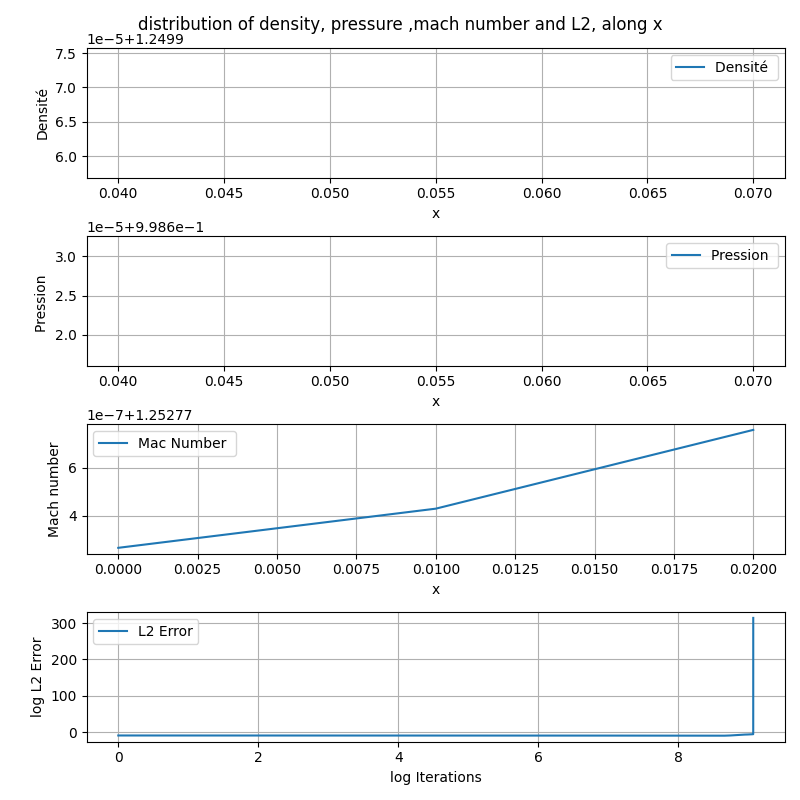
\includegraphics[width=\textwidth,height=\textheight,keepaspectratio]{PLOTS/nozzle_super_super_Beam_CFL020.png}
    \caption{Tuyère supersonic-supersonic at CFL = 0.20}
    \label{fig:your_label}
\end{figure}

\begin{figure}[H] % Use [p] to place the figure on a separate page
    \centering
    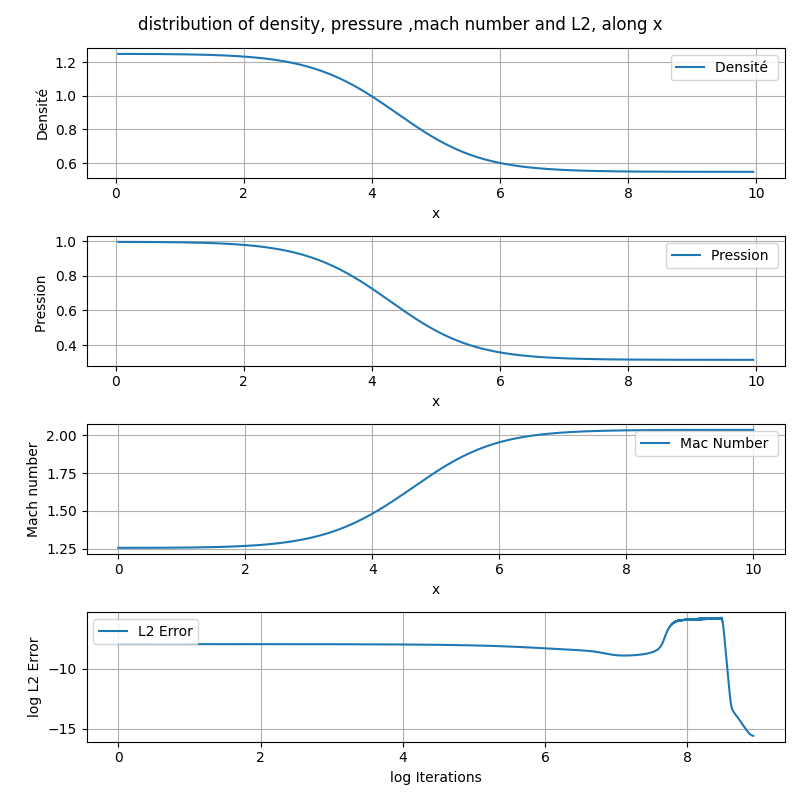
\includegraphics[width=\textwidth,height=\textheight,keepaspectratio]{PLOTS/nozzle_super_super_Beam_CFL060.png}
    \caption{Tuyère supersonic-supersonic at CFL = 0.60}
    \label{fig:your_label}
\end{figure}

\begin{figure}[H] % Use [p] to place the figure on a separate page
    \centering
    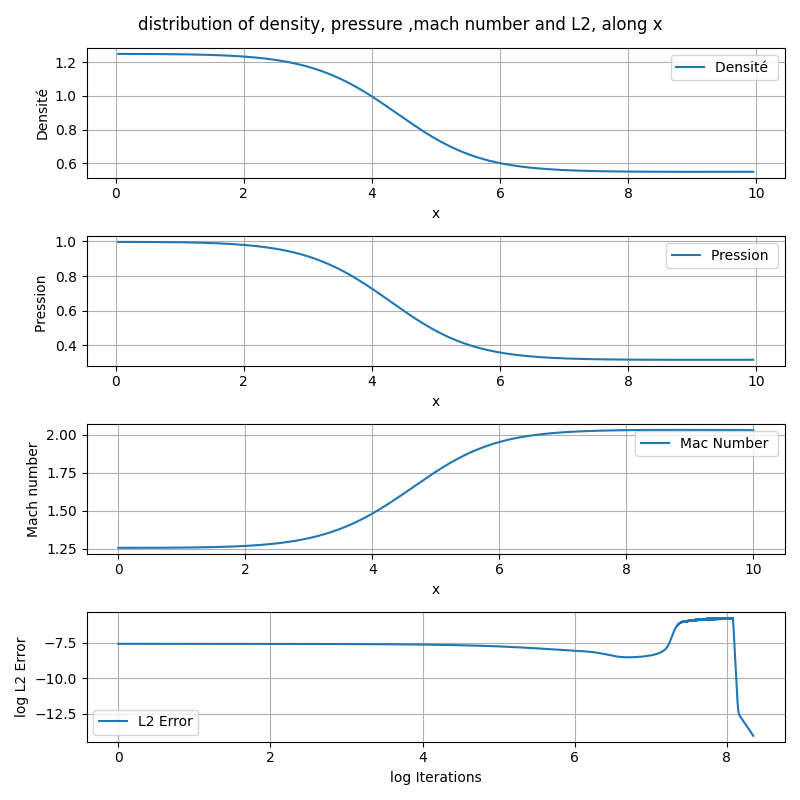
\includegraphics[width=\textwidth,height=\textheight,keepaspectratio]{PLOTS/nozzle_super_super_Beam_CFL110.png}
    \caption{Tuyère supersonic-supersonic at CFL = 1.1}
    \label{fig:your_label}
\end{figure}

\subsubsection{Analysis}

The big surprise here is that the result is different from the macormack method. At the output, we converge to 
Mach 2.00 instead of 1.25 for the macormack. Which is wierd. Futhermore, the simulation diverge at $CFL = 0.2$ but not at
$CFL = 1.1$. The good thing is that we saw some reduction in oscillation at the beam warming method. Futhermore, it is much 
more stable than the macormack method. 

\subsection{SuperSonic - Subsonic nozzles}

\subsubsection{Results}
Unfortunately, the simulation did not work and diverge even if the $CFL = 0.01$ which is really low. We think that the problem
is in the border conditions. I have certainly not implemented the border condition well with the beam warming method. 

\section{Conclusion}
Finally, we explored differents way to simulate a tube choc and the nozzle either on subsonic or supersonic output. The first
way is with the explicit Macmormack method. The second one is with the implicit beam-warming method. The first method tend to be faster 
because there is not matrix operations but tend to be more strict on stability. On the other hand, the beam warming method gives us 
way more flexibility about stability but is more costly to run. Futhermore, the beam-warming method tend to be more stable because there is less oscillation.
this is because the method use dissipative terms. However, we have to be more careful about the Macmormack because we saw that it generate too much oscillations. Therefore,
negatives physics values are generated which make the calculations explode. 

\section{ANNEXE 2: GITHUB LINK}

\href{https://github.com/Kenesis69/MEC_6602E_HOMEWORK_2}{Click for Github Acces}

\end{document}
